\vspace{1em}
{\bf Longwell} is a Web-based RDF browser whose foundational navigation paradigm is faceted browsing. Faceted browsing displays only the properties that are configured to be 'facets' (i.e., to be important for the user browsing data in one or more specific domains) using values for those fields as a means for zooming into a collection by selecting those items with a particular field-value pair.

\begin{figure}
\begin{center}
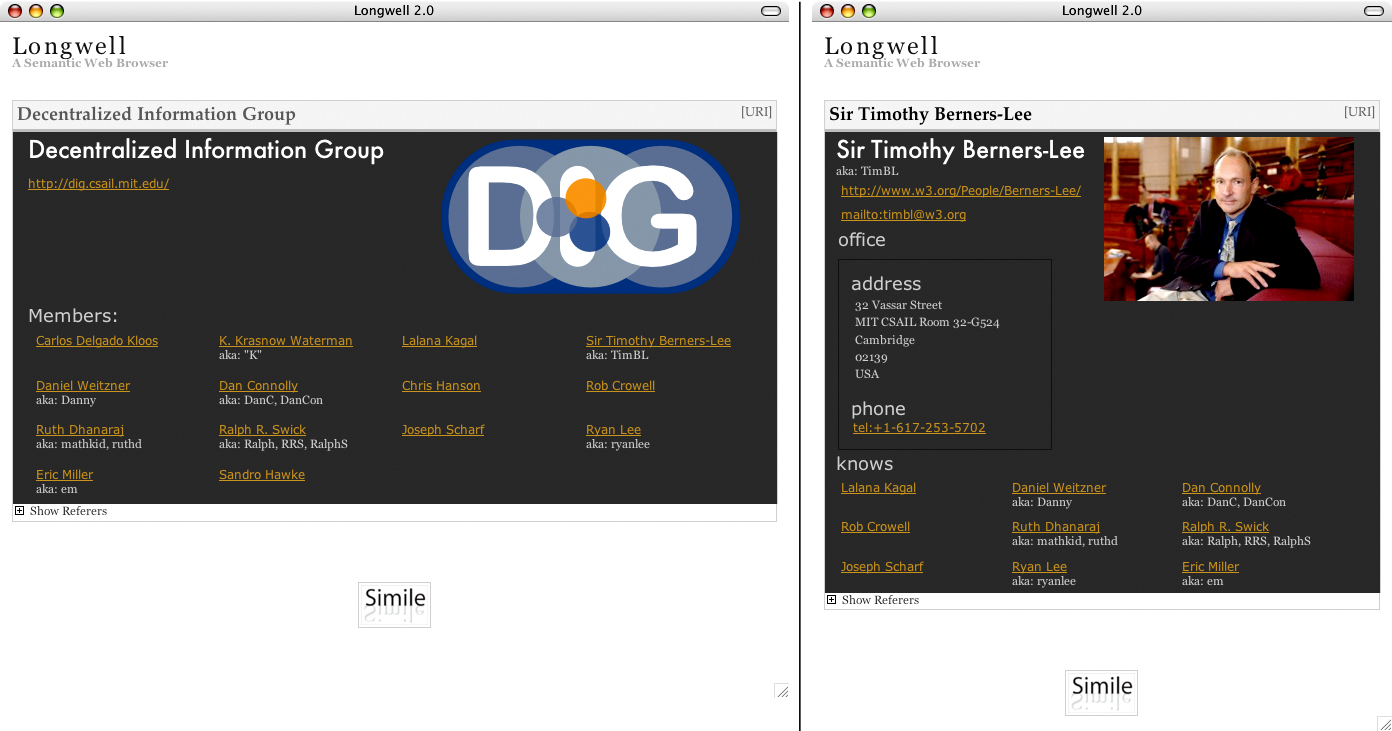
\includegraphics[width=12cm]{longwellScreens.png}
\end{center}
\vspace{-2em}
\caption{Displaying a view of an organization (left) and a constituent member (right) in Longwell}
\label{longwellFig1}
\vspace{-1em}
\end{figure}

The latest version of Longwell relies on the SIMILE Fresnel rendering engine, a Java library built on the Sesame triple store. The engine implements all of the Fresnel core vocabulary and the portion of the extended vocabulary relating to linking groups to CSS stylesheets as well as the option of using FSL as a selector language.
% The emphasis of the Fresnel engine is on building a correct implementation. 
The Fresnel engine output consists solely of an XML representation of the Fresnel lenses and formats as they apply to one resource. Longwell then applies an XSLT transformation to the XML to generate XHTML.  The default XSLT stylesheet shipped with Longwell will generate a traditional nested box layout, as Horus does, but the stylesheet can be modified by XSLT developers to change the model as they see fit.

The left side of Figure \ref{longwellFig1} shows the rendering of a \rdf{foaf:Organization} resource using a lens that gives some details about the organization and lists its constituent members, all \rdf{foaf:Person}s, each listed with their corresponding nickname information to assist in identification.

The nickname list for each person is preceded by the string 'aka: ', added to the display by using the \rdf{fresnel:contentFirst} directive.  The list is also comma separated, accomplished by setting \rdf{fresnel:contentAfter} to a comma.  Clicking on a URI in the display brings the user to that URI; clicking on a textual label changes Longwell's focus to the resource represented by that label.

On the right side of Figure \ref{longwellFig1}, the focus is on one specific member of the organization featured in the left side.  A sublens is used to generate office contact details, and the same sublens used in the organization focus (left image) to describe an organization's members is used in the person focus (right image) to describe who this person claims to know.
